% Fact-checking after ChatGPT exposure: a write-up of the Winter 2025-26 course study
% (Foundations in Psychology and Empirical Study Design, UTN), by Xiaochuan Li,
% 28 Sep 2026. Sources: the group protocol (Assignment 7 and its revised version),
% the pilot table, and my own analysis (Assignment 10, JASP). No raw data are used;
% the Welch tests are computed from the summary statistics by make_figs.py.
% No names of classmates or instructor.
\documentclass[11pt,a4paper]{article}
\usepackage[T1]{fontenc}
\usepackage{newtxtext,newtxmath}
\usepackage[a4paper,margin=2.6cm]{geometry}
\usepackage{graphicx,booktabs,tikz,caption,microtype,array}
\usepackage[round]{natbib}
\usepackage[hidelinks]{hyperref}
\usetikzlibrary{positioning,arrows.meta}
\captionsetup{font=small,labelfont=bf}
\setlength{\parskip}{0.3em}
\definecolor{acc}{HTML}{17457A}
\definecolor{wiki}{HTML}{9AA0A8}

\title{\vspace{-1.2em}\textbf{Does Checking with ChatGPT First Change How People\\Check and Double-Check? A Class Experiment}}
\author{Xiaochuan Li\\[0.2em]\small University of Technology Nuremberg \quad \texttt{xiaochuan.li@utn.de}}
\date{\small Written up September 2026 from a course study, Foundations in Psychology\\ and Empirical Study Design, Winter 2025--26}

\begin{document}
\maketitle

\begin{abstract}
\noindent
This report documents a complete experimental cycle, from design and piloting to revision, online data collection and analysis. Its question: when people can verify an answer with ChatGPT, do they verify more, and do they then look less often at a second source? In a between-subjects experiment, participants answered ten two-alternative general-knowledge questions and could check each answer, first with one tool and then with the other. The first tool was assigned at random: Wikipedia or ChatGPT, shown as static screenshots of each tool's answer. We predicted that the ChatGPT-first group would check more in the first round and less in the second. With 47 participants in the analysis (29 Wikipedia-first, 18 ChatGPT-first), both differences ran against the predictions, and neither was reliable: the ChatGPT-first group checked slightly fewer answers in the first round (5.78 vs.\ 6.24 of 10; Welch $t(29.4) = -0.46$, $p = .65$, $d = -0.15$) and more in the second (7.00 vs.\ 5.38; $t(38.1) = 1.44$, $p = .16$, $d = 0.43$). The study is small and unbalanced, and it measured checking with a fixed, low-cost interface; we report it as a completed pilot-scale experiment, not as evidence for or against the hypothesis.
\end{abstract}

\section{Introduction}
People increasingly hand parts of their thinking to external tools, a practice discussed as \emph{cognitive offloading} \citep{shanmugasundaram}. A review of how digital technology affects cognition discusses over-reliance on AI tools in decision-making, but does not compare AI tools with other digital sources as means of looking up or cross-checking information. A second line of work asks whether ChatGPT functions as an \emph{epistemic authority}: a source whose answer is taken as a reason to believe \citep{hauswald,richards}. Students report treating ChatGPT as a trusted learning source \citep{rastogi}, and educators have raised concerns about what this does to justification practices \citep{cooper,jose}. The study was also prompted by an everyday observation: students verify even simple sums with a calculator, although they were sure of the answer.

We asked whether meeting ChatGPT as the first available checking tool changes checking behaviour, compared with meeting Wikipedia, which is similarly familiar and encyclopaedic. We predicted:
\begin{itemize}\itemsep0em
\item[\textbf{H1}] Participants who can check with ChatGPT first check more of their answers in the first round than participants who can check with Wikipedia first.
\item[\textbf{H2}] Participants who check with ChatGPT first check fewer answers with the other source in the second round.
\end{itemize}
H2 follows the idea that an answer from a tool treated as an authority is less often cross-checked.

\section{Method}
\subsection{Participants}
The class ran the study together, recruiting a convenience sample. Participants had to read English, be familiar with digital search tools, and not be enrolled in advanced courses in psychology or AI. Of 49 participants, two lacked a recorded group assignment and were excluded, leaving 47: 29 in the Wikipedia-first group and 18 in the ChatGPT-first group. The groups are unequal in size; the pilot had revealed a problem with the online group assignment, which was fixed before the main study (Section~\ref{sec:pilot}), and the record does not say why the main groups differ.

\subsection{Materials}
Ten general-knowledge questions each offered two answers (for example, \emph{What is the coloured portion of the eye called?} Iris / Pupil; the full list is in Appendix~\ref{app:items}). For each answer, participants rated their certainty from 1 (\emph{not certain}) to 4 (\emph{highly certain}). The checking tools were presented as static screenshots of Wikipedia's or ChatGPT's answer to the question, so that every participant saw the same content. After the task, participants rated each tool from 1 (\emph{is never correct}) to 4 (\emph{is always correct}), and their usual double-checking from 1 (\emph{I never double-check}) to 4 (\emph{I always double-check}).

\subsection{Design and procedure}
\begin{figure}[t]
\centering
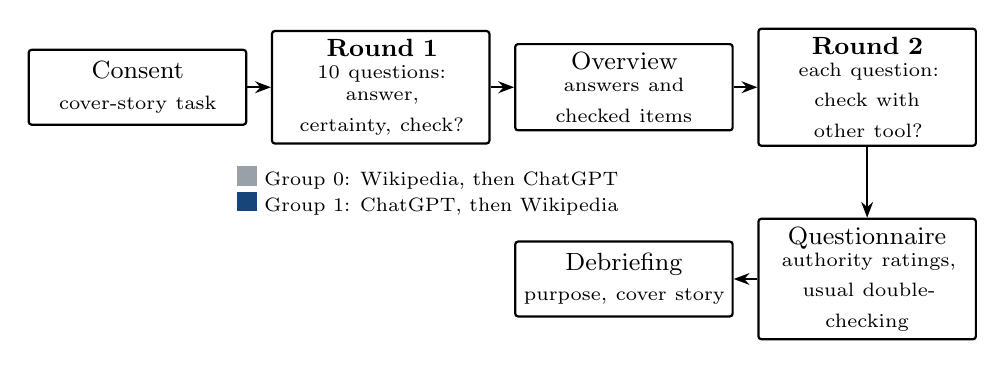
\begin{tikzpicture}[
  box/.style={draw, thick, rounded corners=1pt, minimum height=0.95cm, align=center, font=\small, inner sep=3pt, text width=2.55cm},
  arr/.style={-{Stealth[length=2mm]}, thick}, node distance=0.3cm]
\node[box] (c) {Consent\\\scriptsize cover-story task};
\node[box, right=of c] (r1) {\textbf{Round 1}\\\scriptsize 10 questions: answer,\\\scriptsize certainty, check?};
\node[box, right=of r1] (ov) {Overview\\\scriptsize answers and\\\scriptsize checked items};
\node[box, right=of ov] (r2) {\textbf{Round 2}\\\scriptsize each question:\\\scriptsize check with other tool?};
\node[box, below=0.9cm of r2] (q) {Questionnaire\\\scriptsize authority ratings,\\\scriptsize usual double-checking};
\node[box, left=of q] (d) {Debriefing\\\scriptsize purpose, cover story};
\draw[arr] (c) -- (r1); \draw[arr] (r1) -- (ov); \draw[arr] (ov) -- (r2); \draw[arr] (r2) -- (q); \draw[arr] (q) -- (d);
\node[font=\scriptsize, align=left, below=0.15cm of r1, xshift=0.6cm] (g) {\textcolor{wiki}{\rule{7pt}{7pt}} Group 0: Wikipedia, then ChatGPT\\ \textcolor{acc}{\rule{7pt}{7pt}} Group 1: ChatGPT, then Wikipedia};
\end{tikzpicture}
\caption{Procedure. The first tool (round 1) was assigned at random between subjects; round 2 offered the other tool. A check showed a screenshot of that tool's answer.}
\label{fig:procedure}
\end{figure}

The independent variable was the first available checking tool, manipulated between subjects: group 0 could check with Wikipedia first, group 1 with ChatGPT first (Figure~\ref{fig:procedure}). After giving consent online, participants read a task description that did not mention the checking opportunities. In round 1, they answered each question, rated their certainty, and could check the answer with their group's tool. After an overview of their answers and of which ones they had checked, round 2 offered, for each question, a check with the other tool. The questionnaire followed, asking about the usual double-checking only after the task so that it would not reveal the study's interest. Participants were then debriefed about the cover story and the purpose of the study. The study was anonymous, and no identifying information was collected. It was implemented in PsychoPy and run online through Pavlovia.

\paragraph{Measures.} The two dependent variables are the number of questions checked in round 1 (0--10) and the number checked with the other tool in round 2 (0--10). Round 2 was offered for every question, so its count can include questions that were not checked in round 1; it measures checking with a second source rather than strictly double-checking the same answer.

\subsection{Pilot and revisions}\label{sec:pilot}
Eight people took part in a pilot; seven consented. Although the counterbalancing was set up in PsychoPy and on Pavlovia, six of the eight were assigned to the ChatGPT-first group, and the assignment was then fixed. Participants answered almost all questions correctly and with high certainty, and two did not check any answer, which suggested that the questions were too easy to prompt checking. We therefore replaced two questions with harder ones. One participant noted that a question about the Spanish siesta favoured people with a European background and said they had guessed it; it was among the two replaced. Finally, because one participant rated ChatGPT as almost always correct but checked only with Wikipedia, we added an authority rating for Wikipedia alongside the one for ChatGPT.

\section{Results}
\begin{table}[h]
\centering\small
\begin{tabular}{@{}lcccccc@{}}
\toprule
& \multicolumn{3}{c}{Round 1: first tool} & \multicolumn{3}{c}{Round 2: other tool} \\
\cmidrule(lr){2-4}\cmidrule(l){5-7}
Group & $M$ & $SD$ & Median & $M$ & $SD$ & Median \\
\midrule
Wikipedia first ($n = 29$) & 6.24 & 2.80 & 7.0 & 5.38 & 3.90 & 5.0 \\
ChatGPT first ($n = 18$) & 5.78 & 3.64 & 5.5 & 7.00 & 3.65 & 9.0 \\
\midrule
Predicted & \multicolumn{3}{c}{ChatGPT first higher (H1)} & \multicolumn{3}{c}{ChatGPT first lower (H2)} \\
Observed & \multicolumn{3}{c}{slightly lower} & \multicolumn{3}{c}{higher} \\
\bottomrule
\end{tabular}
\caption{Number of questions checked (of 10). Both scores range from 0 to 10 in both groups.}
\label{tab:desc}
\end{table}

\begin{figure}[h]
\centering
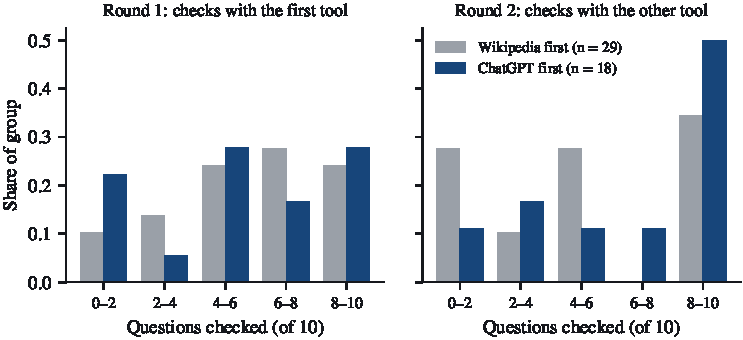
\includegraphics[width=0.92\linewidth]{figs/distributions.pdf}
\caption{Distribution of the number of questions checked, as a share of each group, in the bins of the course analysis.}
\label{fig:dist}
\end{figure}

Table~\ref{tab:desc} and Figures~\ref{fig:dist} and~\ref{fig:means} summarise the two measures. In round 1, the ChatGPT-first group checked slightly fewer answers than the Wikipedia-first group, and its scores were more spread out. In round 2, the ChatGPT-first group checked more answers with the other tool; half of its members checked nine or more of the ten. Round-2 scores clustered at the extremes: many participants checked nearly all answers with the second tool, and in the Wikipedia-first group many checked almost none.

\begin{figure}[h]
\centering
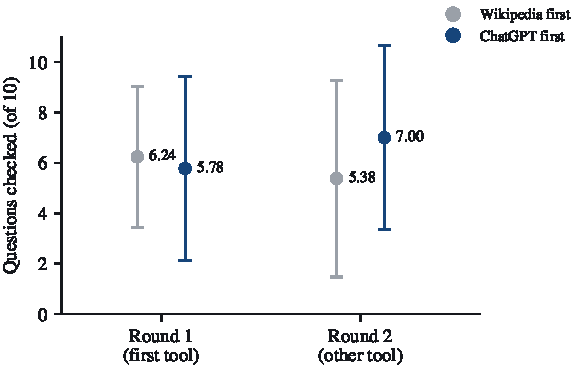
\includegraphics[width=0.5\linewidth]{figs/means.pdf}
\caption{Means $\pm$ one standard deviation.}
\label{fig:means}
\end{figure}

The course analysis was descriptive. For this write-up, we compared the groups with Welch's $t$-test, computed from the summary statistics. Neither difference was reliable. In round 1 the difference was $-0.46$ questions (ChatGPT first minus Wikipedia first), $t(29.4) = -0.46$, $p = .65$, Cohen's $d = -0.15$. In round 2 it was $+1.62$ questions, $t(38.1) = 1.44$, $p = .16$, $d = 0.43$. The scores are bounded counts with skewed distributions, so these tests are a rough guide rather than an exact analysis.

\section{Discussion}
Neither prediction was supported. Descriptively, both differences ran the other way: participants who met ChatGPT first checked slightly fewer answers at first, and checked more answers with Wikipedia afterwards. The second pattern is the larger one, and if it held in a larger sample it would suggest the opposite of the authority hypothesis: that an answer from ChatGPT prompts people to look elsewhere, rather than settling the question. With 18 and 29 participants and effect sizes of this magnitude, however, the study could not tell these patterns apart from chance, and we draw no conclusion about the direction.

\paragraph{Limitations.} The sample was small, unbalanced between groups, and recruited by convenience, largely among students. Checking cost one click and showed a static screenshot, which is much easier than using the real tools; the high rate of checking may reflect this. The questions were easy for many participants even after revision. Round 2 counted checks with the second tool for any question, not only for answers already checked. The certainty and authority ratings were collected but are not analysed here, so we cannot say whether checking tracked uncertainty or trust in a tool. The study was a course exercise without pre-registration or a power analysis.

\paragraph{What a follow-up should change.} A larger, balanced sample; harder questions calibrated so that participants are genuinely uncertain; a checking step with a real cost, such as time; a second round restricted to answers already checked, so that it measures double-checking; and an analysis that relates each check to the rated certainty of the answer and to the rated authority of each tool.

\section*{Contributions and ethics}
I designed the study with two classmates; the class adopted our protocol by vote as the study it would run, and the data were collected by the class. I analysed the data during the course (descriptive statistics in JASP). This write-up, its figures, and the Welch tests computed from summary statistics were prepared by me after the course. Participants gave informed consent online, took part anonymously, and were debriefed about the cover story.

\begin{thebibliography}{9}\small
\bibitem[Cooper et al.(2024)]{cooper} G.~Cooper, K.-S.~Tang, and N.~A.~Rappa. Generative artificial intelligence as epistemic authority? Perspectives from higher education. In H.~Crompton and D.~Burke (Eds.), \emph{Artificial Intelligence Applications in Higher Education}. Routledge, 2024.
\bibitem[Hauswald(2025)]{hauswald} R.~Hauswald. Artificial epistemic authorities. \emph{Social Epistemology}, 39(6):716--725, 2025.
\bibitem[Jose et al.(2025)]{jose} B.~Jose, A.~Cleetus, B.~Joseph, L.~Joseph, B.~Jose, and A.~K.~John. Epistemic authority and generative AI in learning spaces: Rethinking knowledge in the algorithmic age. \emph{Frontiers in Education}, 10:1647687, 2025.
\bibitem[Rastogi and Lawati(2024)]{rastogi} A.~Rastogi and A.~G.~A.~A.~H.~A.~Lawati. Understanding the acceptance of ChatGPT by HEI's students for knowledge enhancement. In \emph{1st International Conference on Innovative Engineering Sciences and Technological Research (ICIESTR)}, pages 1--8. IEEE, 2024.
\bibitem[Richards(2025)]{richards} K.-A.~Richards. Post-cognitive epistemology: Rethinking knowledge, authority, and meaning in the age of predictive language. Working paper, SSRN, 2025.
\bibitem[Shanmugasundaram and Tamilarasu(2023)]{shanmugasundaram} M.~Shanmugasundaram and A.~Tamilarasu. The impact of digital technology, social media, and artificial intelligence on cognitive functions: a review. \emph{Frontiers in Cognition}, 2:1203077, 2023.
\end{thebibliography}

\appendix
\section{Questions}\label{app:items}
\begin{table}[h]
\centering\small
\begin{tabular}{@{}r>{\raggedright\arraybackslash}p{9.2cm}l@{}}
\toprule
& Question & Options \\
\midrule
1 & What is the coloured portion of the eye called? & Iris / Pupil \\
2 & Humans are classified as what species? & Sapiens / Robustus \\
3 & What is the term for when three musical notes are played together? & Chord / Melody \\
4* & What is the largest planet in our solar system? & Jupiter / Saturn \\
5 & What is the name of the art of Japanese paper folding? & Origami / Bonsai \\
6 & What is the famous prehistoric structure on Salisbury Plain, England, called? & Stonehenge / Easter Statues \\
7 & What is the term for nautical miles per hour? & Knot / Speed \\
8 & What are people who make maps called? & Cartographers / Geographers \\
9* & Which metal is liquid at room temperature? & Mercury / Gallium \\
10 & What is the name of the nylon fabric of two pieces that stick to each other, used as a fastener? & Velcro / Toggles \\
\bottomrule
\end{tabular}
\caption{The ten questions after the pilot. Starred questions replaced two pilot items, one of them the question about the siesta.}
\end{table}
\end{document}
